%%%%%%%%%%%%%%%%%%%%%%%%%%%%%%%%%%%%%%%%%%%%%%%%%%%%%%%%%%%%%%%%%%%
%%% Documento LaTeX 																						%%%
%%%%%%%%%%%%%%%%%%%%%%%%%%%%%%%%%%%%%%%%%%%%%%%%%%%%%%%%%%%%%%%%%%%
% Título:		Apéndice A
% Autor:  	Ignacio Moreno Doblas
% Fecha:  	2014-02-01, actualizado 2019-11-11
% Versión:	0.5.0
%%%%%%%%%%%%%%%%%%%%%%%%%%%%%%%%%%%%%%%%%%%%%%%%%%%%%%%%%%%%%%%%%%%%

\pagestyle{fancy}
\fancyhead[LE,RO]{\thepage}
\fancyhead[RE]{Apéndice} %
\fancyhead[LO]{\nouppercase{\rightmark}}

\chapter{Instruction manual}

\minitoc

\section{General}

Welcome to the QRS detection algorithm benchmark platform for integrated and low power devices. This platform is created to make the performance and reliability checks much easier, providing an already implemented environment for testing the user's own algorithm without worrying too much about communications and the measure methods.

This document will guide the user one step at a time in order to accomplish a successful measurement of the algorithm, starting directly with the task of introducing the algorithm into the device.

\section{Introducing the algorithm}
For this task we recommend the usage of Code composer studio, but any IDE capable of compiling and assembling for a Tiva C series (TM4C123GXL) can be used.

There is a lot of stuff inside the project that is not interesting from a user's perspective, which is why the only explanation provided will be of the main files that are needed to introduce the algorithm, grouped in a single folder called “userEntry” and described in the following lines:

\begin{itemize}
    \item \textbf{userAlgorithm.h}: This is the header file, where the helper functions needed to implement the algorithm will be declared. Each one of them have to be placed under the ``User Function'' section. Any function declaration under other sections should not be erased.
    \item \textbf{userAlgorithm.c}: This is the main file where the algorithm will be implemented. One can create any number of helper functions for implementing it, but the main one, which will have the logic of the user's algorithm, needs to be QrsDetectionAlgorithm. This function is the one that will be called by the system. Also there is a function called EcgProcessingConfig that will be called once at the beginning of the benchmark and is perfect for placing all the initializations that the algorithm needs. 
\end{itemize}

All of this can be a little tricky at the beginning but there is a simple example already implemented just for providing a little more help.

\clearpage
\section{Configuring the test environment}
Once the algorithm is implemented in the benchmark device, it is the moment to open the user panel and start configuring the test.

\subsection{Downloading the samples}
This environment is tested with the Mit-BIH arrhythmia database, and ready to work with that data source. A Matlab function is provided with the system to download the desired signal and format it to the application standard. Theoretically, any source can be used as long as it is formatted for the app.

Once the file is created simply add it to the data folder. If it is the first source, the data folder will need to be created. Simply create a folder called “data” at the same level as the app.


\subsection{Configure the benchmark}
According to the image \ref{fig:EndConfigSteps} the configuration of the benchmark only needs 4 steps

\begin{enumerate}
    \item Connect the bench device though the serial port. The device has to be plugged before running the program. Once it is detected, just select it and click start. Ping can be used to check the connection.
    \item Next step is to select the input from one of the data files imported in the previous step. The file is selected simply by clicking on it.
    \item Before running the benchmark the frequency needs to be set. It can be done manually with the knob or automatically by clicking on the read from file button.
    \item Now we are ready to start, just click the Start sending ECG button and the benchmark should begin. For sending a new set of data, just return to the config label and click on the same button. This time the button will be called “Stop sending ECG”.
\end{enumerate}

\clearpage
\section{Interpreting the results}
Using the image \ref{fig:EndResultSteps} as a reference, the information displayed is:

\begin{enumerate}
    \item  A graphic showing the result of the algorithm in real time. The blue line represents the ECG and the red dots the detected R peaks. It can also use a green line that represents the threshold if the algorithm uses one.
    \item Instant frequency, measured between the last two detected beats.
    \item The performance is measured with four different values:
    \begin{itemize}
        \item Processing ticks, that represents the amount of cpu clock ticks used in each operation of the algorithm.
        \item Processing time, uses the processor clock frequency and the previously measured ticks to estimate the same measure in terms of milliseconds.
        \item CPU usage, is an estimation of the percentage of the CPU used, based on the processing ticks used by the algorithm and the data sampling rate.
        \item Memory left, is the minimum amount of stack space that has remained for the task since it was created.  The closer this value is to zero the closer it has come to overflowing its stack.
    \end{itemize}
    \item Annotations table based on the norm UNE-EN 60601-2-47:2002 \cite{Aenor2002}.
    \item Checkboxes to decide if an annotation is taken into consideration for the Reliability or not. All beats found in the database with an unchecked annotation will be treated as an N beat. This is useful for certain algorithms that do not differentiate some types of beats. 
    \item Final measures of reliability, calculated following the guidelines of the norm UNE-EN 60601-2-47:2002 \cite{Aenor2002}.

\end{enumerate}

\begin{figure}[H]
            \centering
                    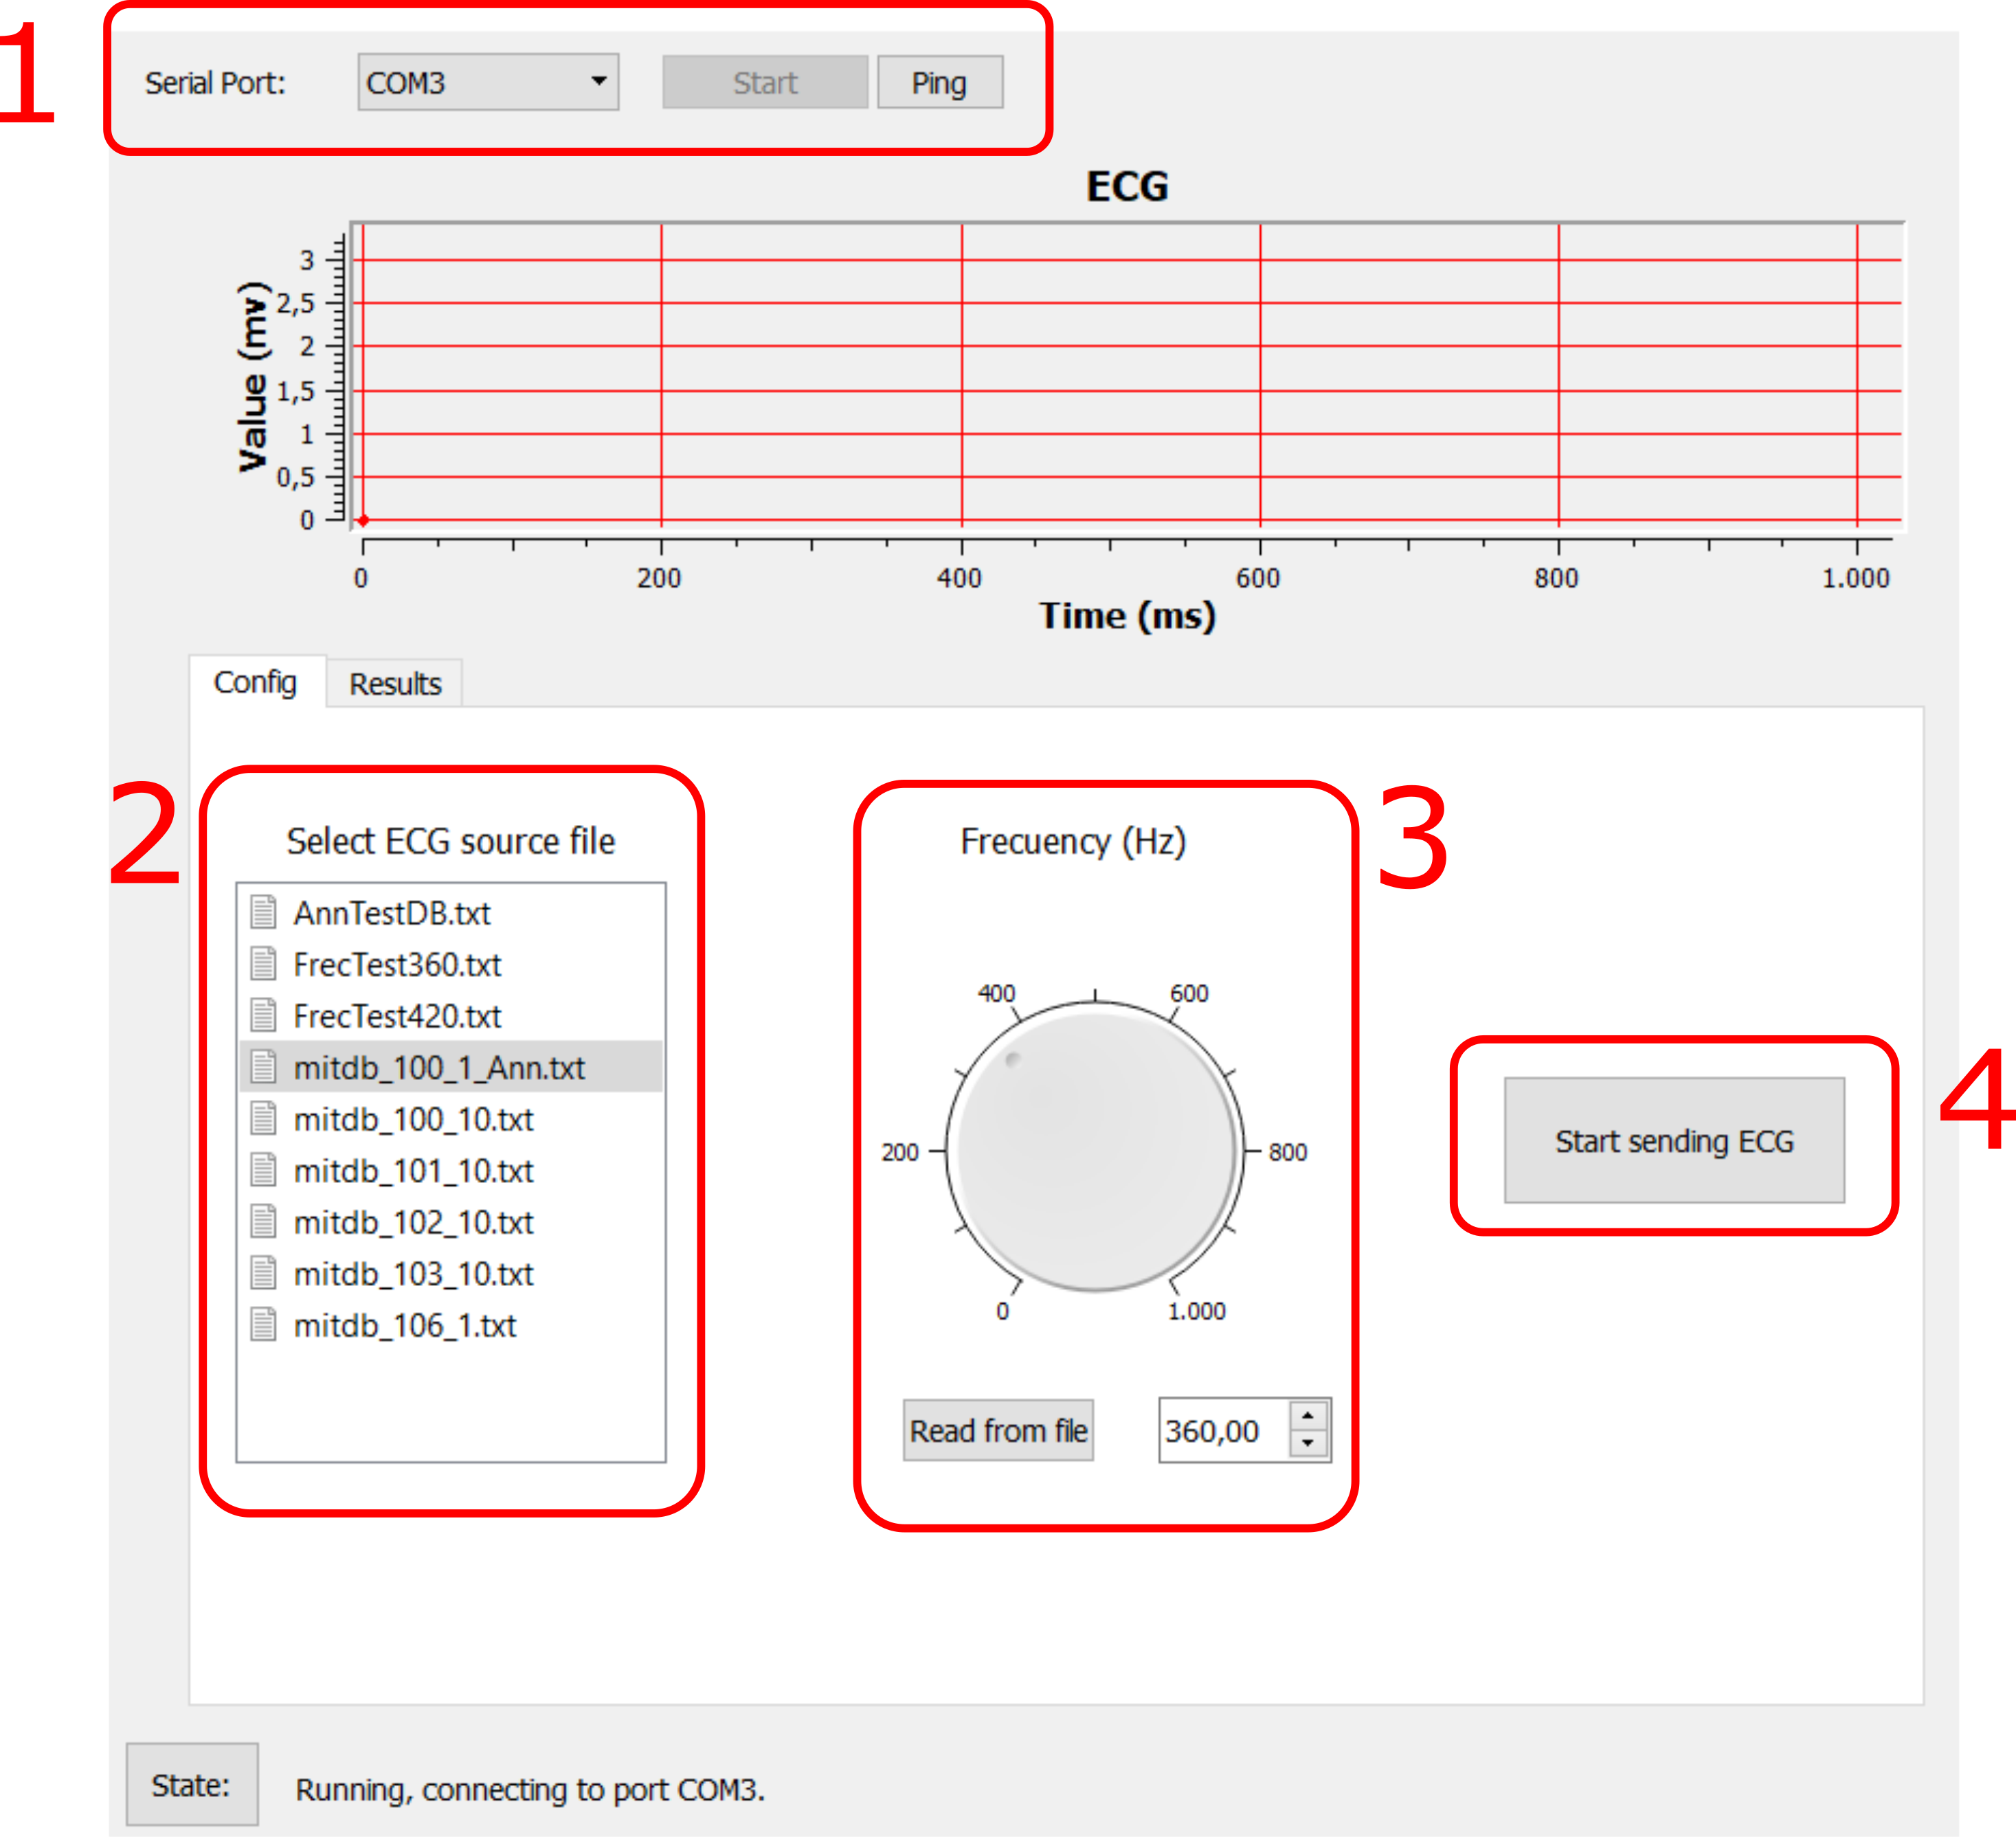
\includegraphics[width = \linewidth]{figuras/configSteps.png}
            \caption{User panel, config label with configuration steps.}
            \label{fig:EndConfigSteps}
        \end{figure}
        
        \begin{figure}[H]
            \centering
                    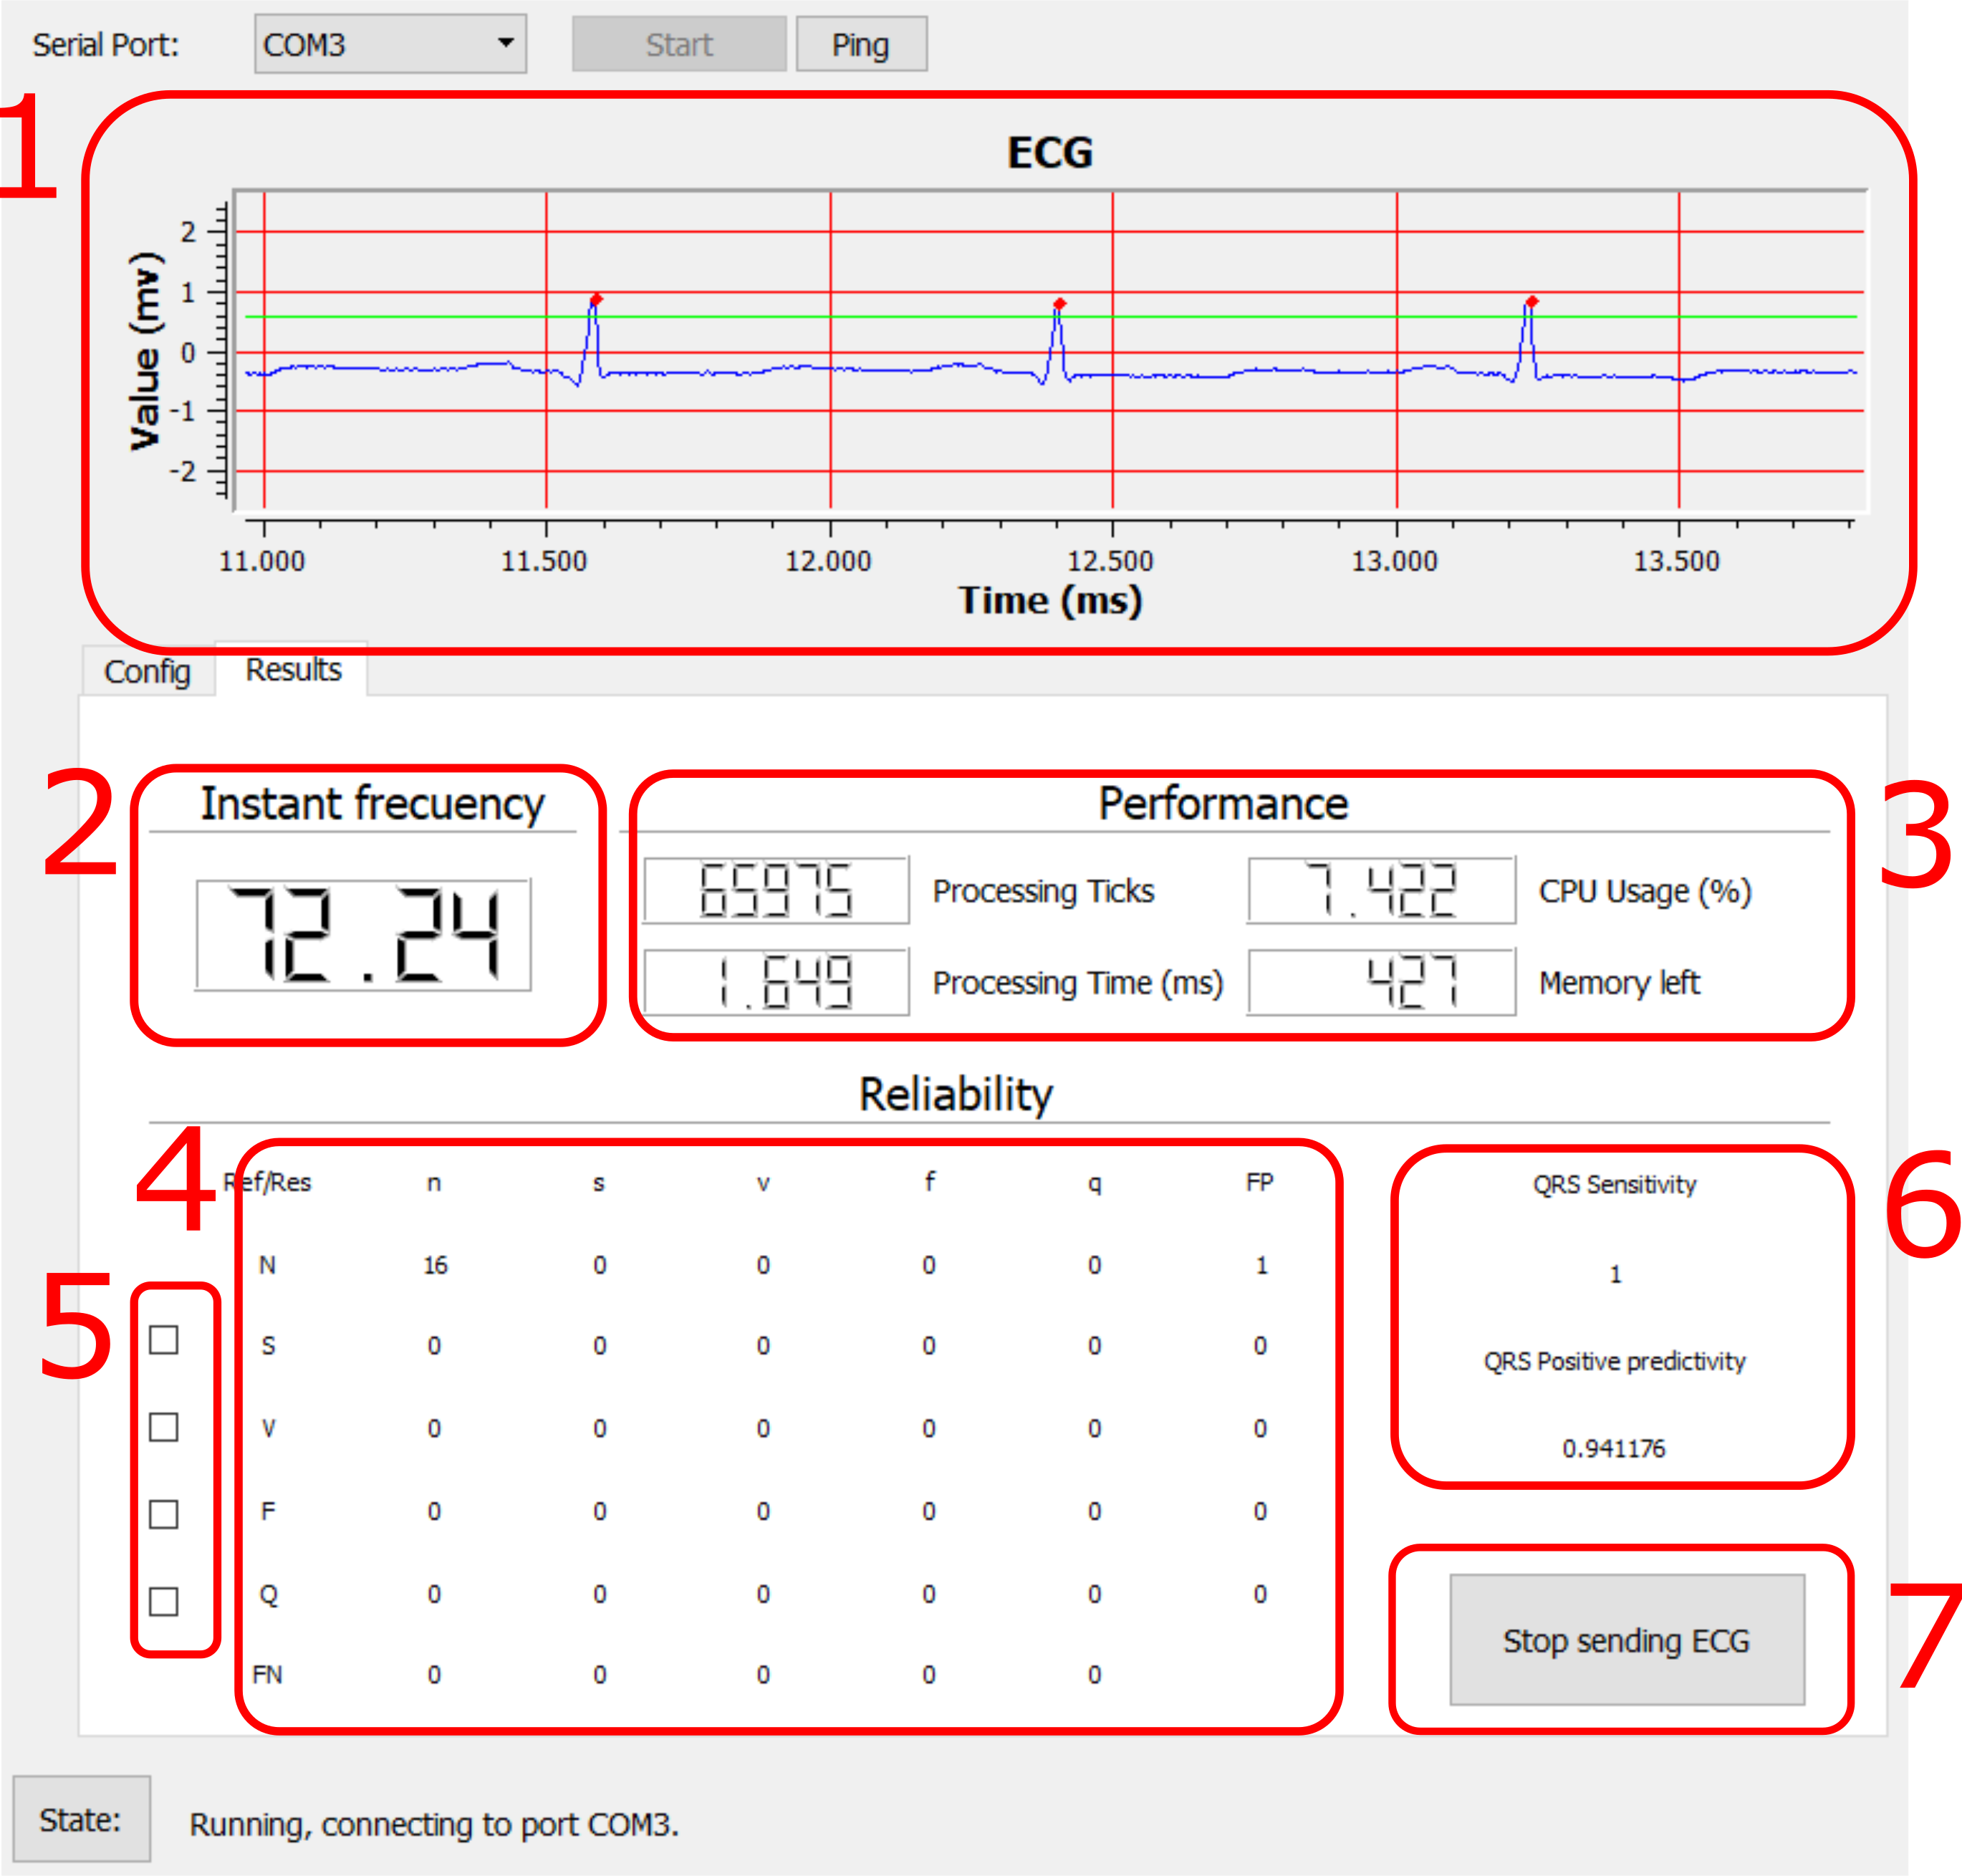
\includegraphics[width = \linewidth]{figuras/resultSteps.png}
            \caption{User panel, result label with helper index.}
            \label{fig:EndResultSteps}
        \end{figure}

\chapterend
